\section{Task 1: Zhengzhou's record and the July 2021 event}\label{sec:q1}

\subsection{Indices and trend model}

We work with nine annual indices computed from the quality-controlled daily series: annual total, wet-day count (days $\ge0.1$\,mm), simple daily intensity (SDII), maximum one-day (Rx1day) and five-day (Rx5day) rainfall, the 95th and 99th percentile exceedance totals (R95p, R99p), and the longest dry and wet spells. Trends are estimated with the non-parametric Sen slope \cite{sen1968}, tested with the Mann--Kendall statistic \cite{mann1945}, and a change point is searched with the Pettitt test \cite{pettitt1979} on the sign-based statistic $U_t$, which avoids the inflated significance that the rank-sum variant produces on a series with a strong seasonal-free but skewed distribution.

For counts of threshold exceedances we use a Poisson generalised linear model with a log link and a linear time term, because a count is not a continuous variable and the Sen slope on counts is only descriptive.

\subsection{Results}

Table~\ref{tab:q1trend} reports the 1961--2020 trends. The remarkable feature is not a trend in total rainfall but the joint behaviour of frequency and intensity: wet days fall by 2.0 days per decade ($p=0.021$, robust to false-discovery control) while SDII rises by 0.23\,mm\,dec$^{-1}$ ($p=0.062$) and the number of days above 100\,mm rises by 14.9\% per decade ($p=0.343$). The total is flat (+1.19\,mm\,dec$^{-1}$, $p=0.92$) because the increase in intensity and the decrease in frequency offset each other. This is a textbook signature of a rainfall regime becoming more concentrated, and it is precisely the regime in which a stationary design standard fails.

\begin{table}[H]
\centering
\caption{Zhengzhou annual indices, 1961--2020 ($n=53$): Sen slope, Mann--Kendall $p$, and Poisson trend for counts.}
\label{tab:q1trend}
\small
\begin{tabular}{lrrrr}
\toprule
Index & Mean & Sen slope & MK $p$ & 95\% CI of slope\\
\midrule
Total (mm) & 642.5 & $+1.19$ & 0.921 & $[-22.94,\,27.74]$\\
Wet days (d) & 81.6 & $-2.00$ & 0.021 & $[-3.80,\,-0.29]$\\
SDII (mm\,d$^{-1}$) & 7.87 & $+0.234$ & 0.062 & $[-0.016,\,0.482]$\\
Rx1day (mm) & 82.7 & $+0.449$ & 0.824 & $[-4.29,\,5.58]$\\
Rx5day (mm) & 122.7 & $+3.74$ & 0.357 & $[-4.74,\,10.41]$\\
R95p (mm) & 236.9 & $-4.13$ & 0.495 & $[-16.19,\,8.95]$\\
R99p (mm) & 85.3 & $+0.578$ & 0.812 & $[-4.86,\,6.04]$\\
\midrule
Days $\ge25$\,mm & -- & $+1.5\%$\,dec$^{-1}$ & 0.589 & --\\
Days $\ge50$\,mm & -- & $-2.0\%$\,dec$^{-1}$ & 0.705 & --\\
Days $\ge100$\,mm & -- & $+14.9\%$\,dec$^{-1}$ & 0.343 & --\\
\bottomrule
\end{tabular}
\end{table}

The Pettitt test finds no significant break in either the total ($K=144$, candidate year 2002, $p=0.88$) or Rx1day ($K=97$, candidate 2004, $p=1.00$). We therefore keep a stationary baseline for the return-level calculation and treat any apparent shift as sampling noise; this decision is revisited in Section~\ref{sec:q3}, where a non-stationary variant is tested on held-out data and found to improve levels but not ranks.

\begin{figure}[H]
\centering
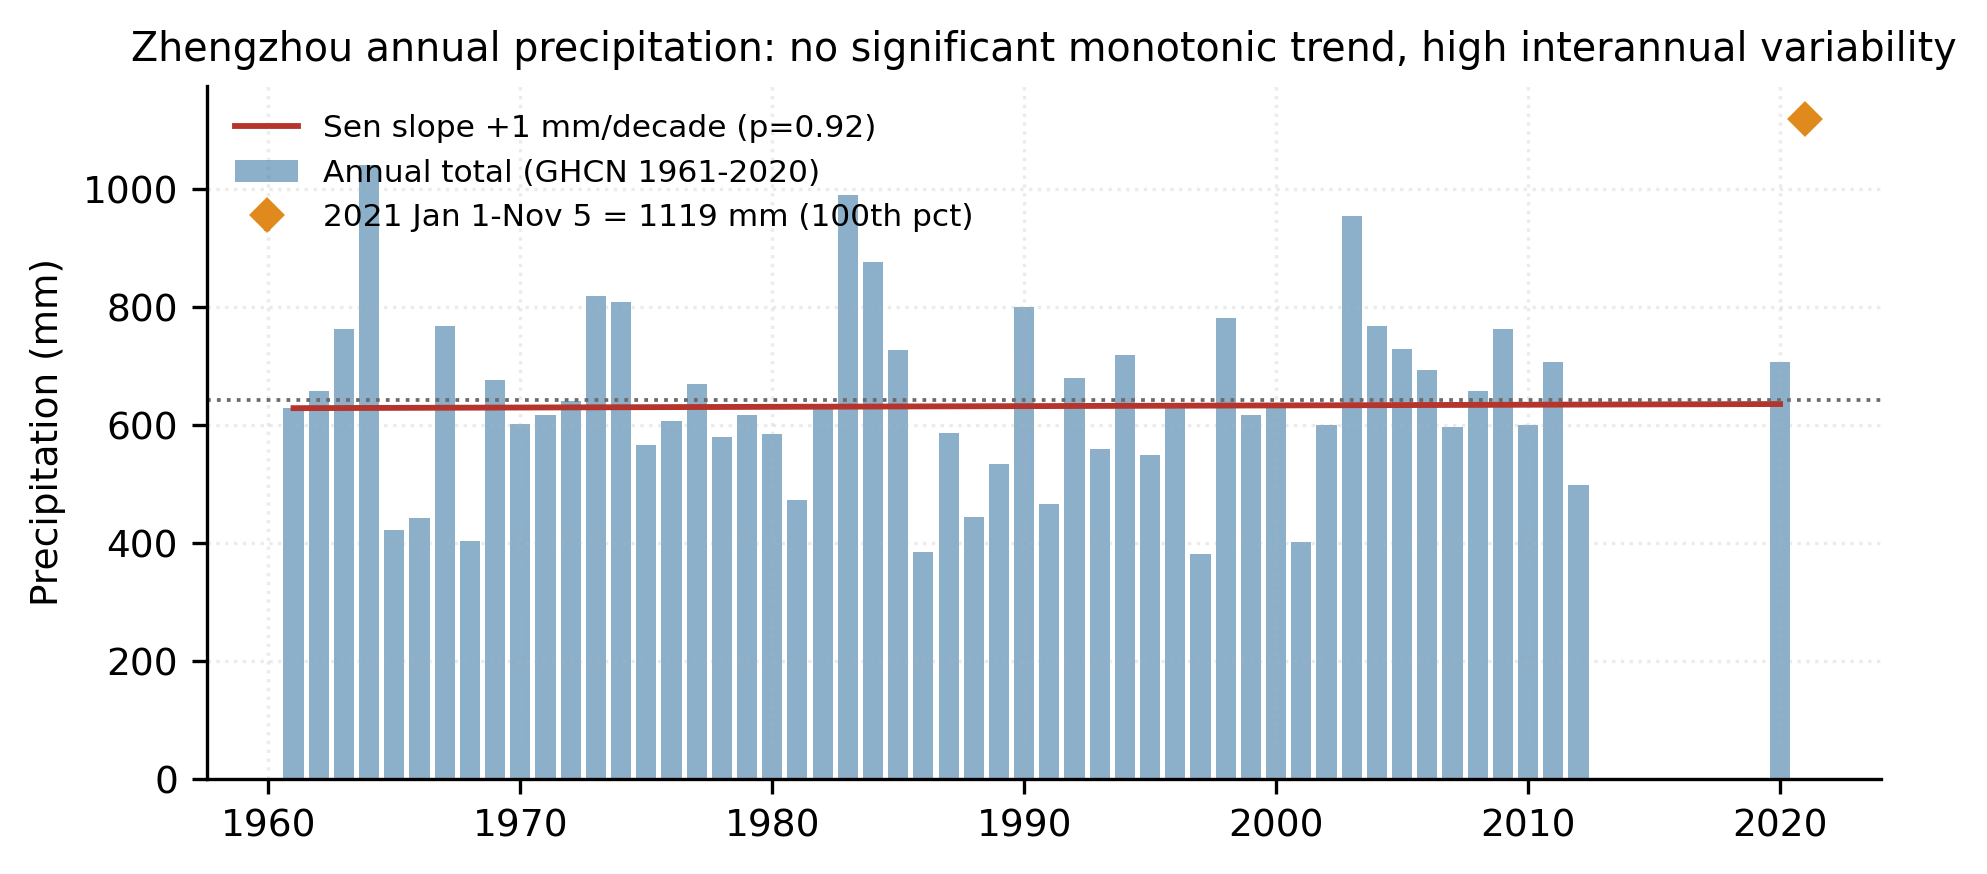
\includegraphics[width=0.42\linewidth]{../02_figures/fig01_annual_total.png}
\caption{Annual precipitation at Zhengzhou, 1951--2024. The Sen line is fitted on 1961--2020; the 2021 diamond (1\,119.4\,mm for January--5 November) lies far above the fitted distribution of the 53 complete years.}
\label{fig:annual}
\end{figure}

\subsection{Return levels and the rarity of the event}

A generalised extreme value distribution $F(x)=\exp\{-[1+\xi(x-\mu)/\sigma]^{-1/\xi}\}$ \cite{coles2001} is fitted by maximum likelihood to the 53 annual daily maxima of 1961--2020; the shape estimate is $\xi=-0.026$, i.e.\ a light upper tail close to the Gumbel case, and Section~\ref{sec:eval} shows how little this parameter is identified. Confidence intervals come from a parametric bootstrap with 1\,000 replicates for the return levels and 500 (300 for the official 449\,mm) for the event return periods, with a fixed seed. Table~\ref{tab:q1rl} gives the return levels.

\begin{table}[H]
\centering
\caption{Return levels of daily precipitation at Zhengzhou (mm), GEV fitted on 1961--2020, with bootstrap 95\% intervals.}
\label{tab:q1rl}
\footnotesize
\setlength{\tabcolsep}{3pt}
\begin{tabular}{lrrrrrr}
\toprule
$T$ (yr) & 2 & 5 & 10 & 20 & 50 & 100\\
\midrule
Level (mm) & 78.0 & 106.3 & 124.5 & 141.7 & 163.4 & 179.4\\
95\% CI & [69.3, 87.0] & [95.1, 118.6] & [109.1, 140.5] & [120.3, 165.3] & [132.0, 204.7] & [139.2, 242.5]\\
\bottomrule
\end{tabular}
\end{table}

The 20 July 2021 daily total of 188.7\,mm exceeds the 100-year level. Its empirical return period, read from the 54 complete years that precede it, is 54\,yr; the fitted GEV assigns 151\,yr. The difference is instructive: an event of this size was not unprecedented in the daily record (1978 reached 189.4\,mm), so a naive daily analysis would classify 2021 as rare but plausible and stop there. The three-day total of 313.4\,mm is another matter: it is the largest in 71 years of record, and the fitted three-day GEV places it at $6.4\times10^{3}$\,yr. For the official three-day total of 449\,mm the fitted model returns $1.6\times10^{8}$\,yr, reported only to make a point: above roughly the 200-year level the extrapolation is dominated by the uncertain shape parameter, and the interval spans 678\,yr to infinity. The honest statement is that 449\,mm in 72\,h lies outside the range in which a 53-year record can discriminate between return periods; the practical conclusion does not depend on the exact number, because the event exceeded every standard in force by a factor of three or more.

\subsection{Wet years}

The five wettest years in 1961--2020, expressed as standardised anomalies, are 1964 (1\,041.3\,mm, $z=2.69$), 1983 (990.6\,mm, $z=2.35$), 2003 (953.9\,mm, $z=2.10$), 1984 (877.4\,mm, $z=1.58$) and 1973 (819.6\,mm, $z=1.19$). Their spacing is irregular, consistent with the absence of a change point: wet years are a stationary tail phenomenon, not a regime. The 2021 year, even truncated at 5 November, reaches 1\,119.4\,mm ($z=3.46$) and is the wettest year in the 71-year GHCN record.

\subsection{Quantifying the waterlogging event}

Rainfall becomes a disaster through runoff. We estimate the storm-water volume with the SCS curve-number method \cite{neh1986}, $Q=(P-0.2S)^2/(P+0.8S)$ with $S=25400/\mathrm{CN}-254$, applied to the 1\,180\,km$^2$ built-up area of Zhengzhou. Antecedent wetness in July 2021 was high, so we bracket the curve number between 75 and 95; the central case is CN\,85, appropriate to a dense urban surface with partial sewer connection. Over the event window the areal rainfall is 313.4\,mm, giving a runoff depth of 265.4\,mm and a volume of $3.13\times10^{8}$\,m$^3$; at the official 449\,mm the volume is $4.71\times10^{8}$\,m$^3$. Table~\ref{tab:cn} shows the sensitivity.

\begin{table}[H]
\centering
\caption{Runoff response of the 1\,180\,km$^2$ urban area to the July 2021 storm (SCS-CN).}
\label{tab:cn}
\small
\begin{tabular}{lrrrrr}
\toprule
Curve number & 75 & 80 & 85 & 90 & 95\\
\midrule
Runoff depth (mm) & 230.6 & 248.3 & 265.4 & 281.9 & 297.9\\
Volume ($10^{8}$\,m$^3$) & 2.72 & 2.93 & 3.13 & 3.33 & 3.52\\
\bottomrule
\end{tabular}
\end{table}

The failure mechanism is a capacity mismatch in time, not in volume alone. The peak hour delivered 201.9\,mm\,h$^{-1}$; the one-year design intensity of the Zhengzhou network is about 36\,mm\,h$^{-1}$, the two-year 43 and the three-year 50. The peak therefore exceeded design capacity by factors of 5.6, 4.7 and 4.0. Routing that hour through the same curve-number model gives 156.6\,mm of runoff, of which 120.6\,mm lies above the one-year capacity --- $1.4\times10^{8}$\,m$^3$ arriving within sixty minutes. Clearing the three-day event (313.4\,mm of rain, 265.4\,mm of runoff) at full capacity takes 7.4\,h at the one-year standard and 5.3\,h at the three-year standard, and during that time surface water continues to accumulate in underpasses, basements and the metro. This is why the loss was concentrated in underground space: the network was not merely overloaded, it was overloaded for a full working day. The daily structure of the event, its monthly context and its return periods are plotted in Appendix~\ref{app:extrafig}.
